%%%---------------------------------------------------------------%%%
%%% Wyzsza Szkola Gospodarki Bachelor's Thesis                    %%%
%%% Prepared by Bruno Axel Kamere                                 %%%
%%% Inspired by Artur M. Brodzki & Piotr Woźniak's WUT template.  %%%
%%% Computer Engineering and Mechatronics Department              %%%
%%% Wyzsza Szkola Gospodarki w Bydgoszczy, 2022                   %%%
%%%---------------------------------------------------------------%%%

\documentclass[
    left=2.5cm,         % Sadly, generic margin parameter
    right=2.5cm,        % doesnt't work, as it is
    top=2.5cm,          % superseded by more specific
    bottom=3cm,         % left...bottom parameters.
    bindingoffset=6mm,  % Optional binding offset.
    nohyphenation=false % You may turn off hyphenation, if don't like.
]{config/classes/config-thesis}

\raggedbottom % Don't stretch text.
%--------------------------------
% Use English language (Other languages to be added in the future)
%--------------------------------
\langeng

%--------------------------------
% Image path
%--------------------------------
\graphicspath{
    {img/}
    {30. introduction/figures/}
    {40. chapter 1 - theory/figures/}
    {50. chapter 2 - technique and approach/figures/}
    {60. chapter 3 - setup/figures/}
    {70. discussion/figures/}
    {80. conclusion/figures/}
}

%--------------------------------
% Reference the bibliography file
%--------------------------------
\addbibresource{bibliography.bib}


%%%---------------------------------------------------------------%%%
%%% Start main document                                           %%%
%%%---------------------------------------------------------------%%%
\begin{document}

\EngineerThesis
\universityname{UNIVERSITY OF ECONOMY IN BYDGOSZCZ}
\institute{Informatics and Mechatronics}
\field{Computer Engineering and Mechatronics}
\course{Mechatronics}
\title{Cloud Managed Unmanned Aerial System}
\author{Bruno Axel Kamere}
\studentnumber{030756}
\seminarlecturer {Szychta Elżbieta, prof. dr hab. inż.}
\supervisor{Ocetkiewicz Tomasz, mgr inż.}
\date{\the\year}
\maketitle
\frontmatter

%--------------------------------
% Dedication
%--------------------------------
% ******************************* Thesis Dedication ********************************
% \cleardoublepage

\begin{dedication}

    This work is dedicated to my loving and very supportive parents \dots

\end{dedication}

%--------------------------------
% Acknowledgements
%--------------------------------
% ************************** Acknowledgements **************************
\cleardoublepage

\section*{\centering \Large Acknowledgements}

\begin{acknowledgements}

    Looking back at my journey that led to this point, I would like to take some time and thank everyone that has helped me throughout my studies, and design, development, and testing of this final engineering work. The moral support received throughout this period is unprecedented.

    I would like to first and foremost thank my lovely parents. They have been there for me in each single step that led to where I am and what I have achieved today. They have encouraged me, believed in me, and supported me in various ways. Thank you.

    Next, I would like to also thank a lot my thesis supervisor, Ocetkiewicz Tomasz, mgr inż.; first, for believing in my ability to conduct my research towards the execution of my project and second, for the unprecedented advice and support I have received throughout my studies and throughout my final engineering research and project execution. Thank you.

    I want to also take a moment to thank the WSG university’s institute of informatics and mechatronics professors and staff for the knowledge and skills they have provided me throughout my studies. They have inspired me to like more my field of studies, due to the challenges provided to me along the way. Thank you.

    Finally, I would not finish without thanking my classmates, colleagues and friends who have been part of my support system and have given me ideas and support during throughout my studies, until this day. A big thanks to you.


\end{acknowledgements}



%--------------------------------
% Abstract
%--------------------------------
\cleardoublepage
\abstract
\lipsum[1-3]
\keywords AWS, UAV, UAS

%--------------------------------
% Declaration of author's will
%--------------------------------
\newpage
\pagestyle{plain}
\makeauthorship

%--------------------------------
% Table of Contents
%--------------------------------
% \cleardoublepage
\clearpage
\tableofcontents


%--------------------------------
% List of Figures
%--------------------------------
% \cleardoublepage
\clearpage
\listoffigures
% \listoffigurestoc

%--------------------------------
% List of Tables
%--------------------------------
% \cleardoublepage
\clearpage
\listoftables
% \listoftablestoc

%--------------------------------
% List of Listings
%--------------------------------
% \cleardoublepage
\newpage
\listoflistings

%--------------------------------
% Nomenclature
%--------------------------------

\printnomenclature
% \acronymlist

\mainmatter
%--------------------------------
% Chapters - Introduction
%--------------------------------
\cleardoublepage
\pagestyle{headings}
% ------------------------------------------------------------------------
% 30. Introduction
% ------------------------------------------------------------------------

\chapter{Introduction}
\label{cha:thesis-introduction}

Unmanned Aerial Vehicles also known as UAVs or Drones, although hardly a new technology, with the first used UAV recorded in history dating back to 1849~\cite{vasileprisacariujdrm2017}, have recently gained a lot of attention from various sectors ranging from entertainment to military. This is going to have an impact that cannot be overseen over the coming years as more and more people find uses of UAVs in various applications. UAVs were initially developed to be used for military operations, mainly surveillance, but they were later armed to also enable them to perform long-distance military operations without putting humans at risk. The United States of America has used these types of UAVs mainly in the wars in the Middle East, where UAVs like the General Atomics MQ-9 Reaper also known as Predator B and Northrop Grumman RQ-4 Global Hawk have been widely deployed~\cite{samaanorientxxi2022}.

Despite their use in the military sector, UAVs have also been employed in other sectors such as commercial and entertainment sectors, where UAVs are being used in things like land geography mapping, industrial surveillance, photography and many more. Companies like SZ DJI Technology Co., Ltd. or Shenzhen DJI Sciences and Technologies Ltd. in full, more popularly known as its trade name DJI have had a lot of success in this area, where as of March 2021 DJI was coveringitself covers (research on the percentage of drones that DJI makes and are on the market). UAVs have also seen great use in the healthcare sector, where companies like Zipline~\cite{droneslevy2022} are implementing an end-to-end supply chain system that employs UAVs to supply and deliver medical supplies to hospitals in rural areas in Rwanda that are hard to reach or inefficient to reach by other means of delivery.

Rwanda has also seen great use of UAVs during the COVID-19 pandemic where UAVs were widely used by the Rwanda’s Ministry of Health and the Rwanda National Police to spread COVID-19 awareness in Kigali communities~\cite{whoafricarw2020}.

As UAVs gain the market, the need to have robust UAV systems also known as UASs becomes eminent. Therefore, in this thesis, focus was put in designing and building a robust, scalable, highly available cloud deployed Unmanned Aerial System, that can easily be integrated with cloud services like Amazon Web Services also known as AWS to provide a solution where UAV pilots can control UAVs from virtually anywhere in the world. The proposed system comprises of a UAV flying with onboard compute that has an LTE datalink to a ground control system also known as GCS, dashboards and a command-and-control center application running in a highly available and fault tolerant AWS cloud infrastructure. The focus of this thesis is to therefore assess the possibilities of implementing such a solution in an efficient, resilient, reliable, and highly available manner and discuss on the pros and cons of the solution.

The proposed solution, as seen in the high high level design in figure \ref{fig:uas-hhld}, was developed following the best industry standards in software development and architecture as is going to be described in detail in the next chapters. This thesis is also going to discuss the developments that have already been made in this area as well as areas that need further research and development.

\begin{figure}[!h]
    \centering 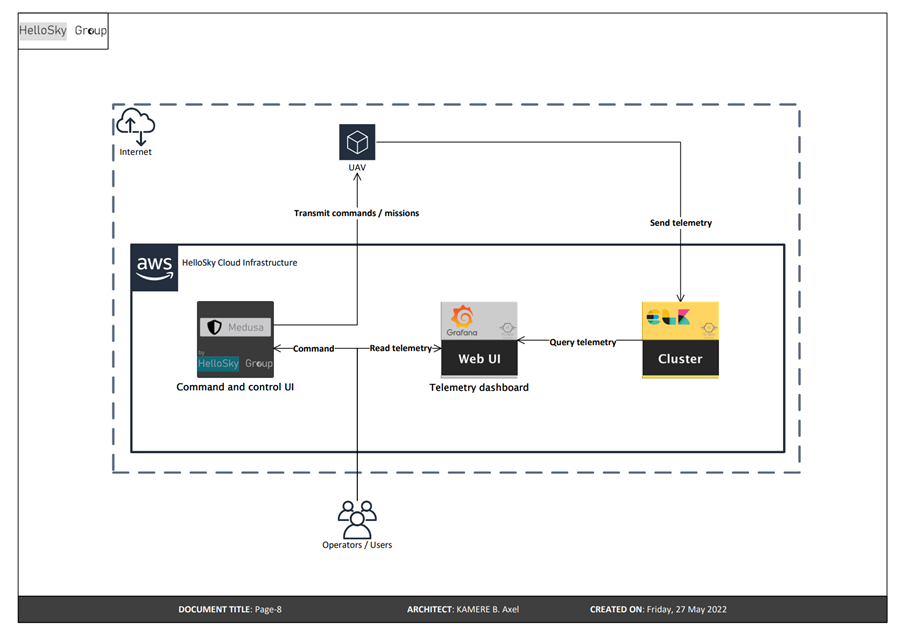
\includegraphics[width=1\linewidth]{UAS HHLD.png}
    \caption{System High High Level Design.}
    \label{fig:uas-hhld}
    \source{Own creation. Designed with Microsoft Visio. Refer to \ref{subsec:ms-visio}.}
\end{figure}


\section{Related work}
\label{sec:related-work}

UAVs and UASs in general is a field that has undergone substantial development through various researches done by scientists, engineers and academicians.

One of the challenges faced by UAVs, especially in the capability of being able to deploy them in urban areas is the safety of their operations. Being able to build a UAV with highly effective collision avoidance algorithms is a still a field under active research. And this is one of the main challenges that need to be solved for the world to see robust autonomous UAVs employed widely in communities for various use cases. Pedro et. al have studied on how UAVs can be made more resiliant and safe with the help of artificial intelligence, machine learning and the likes. In their article "Framework for fully autonomous UAVs"~\cite{Pedro2020}, they reviewed the current collision avoidance algorithms for both static and dynamic objects and proposed a conceptual framework to improve more the safety and realiability of UAVs.
%---------------------------------1.1 Use case---------------------------------%
\section{Use case}
\label{sec:use-case}

As UAVs emerge, there will be a need to be able to centrally manage a fleet of UAVs. Depending on the UAV use case, operators might need to also control them at a long distance beyond eyesight. A UAV operates as part of a system comprised of multiple other components that support the operation of a UAV. The main components are a Ground Control System, (Research on the main components of a UAV). UAVs can either be Fully autonomous, fully manual, or semi-autonomous. UAVs can also be employed in various use cases, below are various scenarios in which UAVs can be used
\begin{itemize}
    \item Terrain mapping.
    \item Shipping and delivery.
    \item Search and rescue.
    \item Law enforcement.
    \item Military reconnaissance / Surveillance.
\end{itemize}

For a UAV to perform any of the above, it needs to meet certain criteria, a UAV should:
\begin{itemize}
    \item Have onboard computer to process mission commands on the fly.
    \item Have onboard key components like,
          \begin{itemize}
              \item Sensors, depending on the mission.
              \item Cameras.
              \item Battery.
              \item LTE modules or Satnav modules to allow communication with ground control.
          \end{itemize}
    \item Have LTE or Satellite communication to enable the UAV to set up a datalink with the ground control. The UAV would have to send data such as
          \begin{itemize}
              \item	Ground speed.
              \item	Altitude.
              \item	Battery levels.
              \item	Yaw.
              \item	Location.
              \item	Direction.
              \item	Sensor data.
              \item	Send the data frequently for real-time or near real-time communication.
              \item	Be able to react and if necessary, take evasive maneuvers when:
                    \begin{itemize}
                        \item On collision course.
                        \item The batteries are low on power.
                        \item Out of connectivity range.
                    \end{itemize}
          \end{itemize}
\end{itemize}


%---------------------------------1.2 Problem definition---------------------------------%
\section{Problem definition}
\label{sec:problem-definition}


%---------------------------------About HelloSky Group---------------------------------%
\section{About HelloSky group}
\label{sec:about-hellosky-group}

Across this thesis, there will be mentions of the name "HelloSky group". Several designs built for the project as well as source codes all have mentions of HelloSky group or hsg in abbreviations.

HelloSky group is a company name that I came up with to brand my work done and future developments that will be made on this project and many other related projects that will be built in the future. HelloSky group in itself was though as a group company that will have multiple child companies, and in the scope of this project, it will be used to represent the part of the company that is envisioned to deal with aerial monility, hence being the scope of the thesis. Figure \ref{fig:hs-group-logos} shows the HelloSky group logos used throughout the thesis project.

\begin{figure}[!h]
    \centering
    \begin{subfigure}{0.4\textwidth}
        
\includegraphics[width=\linewidth]{hs_group_wide_500x200.png}
        \caption{Colored 500 x 200.}
        \label{fig:hs-group-wide-500x200}
    \end{subfigure}
    \hspace*{\fill}
    \begin{subfigure}{0.4\textwidth}
        
\includegraphics[width=\linewidth]{hs_group_wide_dark_500x200.png}
        \caption{Black and white 500 x 200.}
        \label{fig:hs-group-wide-dark-500x200}
    \end{subfigure}
    \caption{HelloSky group logos.}
    \label{fig:hs-group-logos}
    \source{Own creation. Designed with Affinity Designer. Refer to \ref{subsec:affinity-designer}.}
\end{figure}


\nomenclature[z-UAV]{UAV}{Unmanned Aerial Vehicle}
\nomenclature[z-UAS]{UAS}{Unmanned Aerial System}
\nomenclature[z-GCS]{GCS}{Ground Control Station}
\nomenclature[z-LTE]{LTE}{Long Term Evoluton (Telecommunication)}
\nomenclature[z-DJI]{DJI}{Da-Jiang Innovations}
\nomenclature[z-AWS]{AWS}{Amazon Web Services}
\nomenclature[z-HLD]{HLD}{High Level Design}
\nomenclature[z-HHLD]{HHLD}{High High Level Design}

%--------------------------------
% Chapters - Theory
%--------------------------------
\cleardoublepage
% ------------------------------------------------------------------------
% 40. Theory
% ------------------------------------------------------------------------

\chapter{Theory}

In this chapter, key background concepts and methodologies used in the thesis are going to be discussed. The chapter is going to discuss explain what is meant by unmanned aerial system and its components.

The chapter is also going to discuss on the cloud provider, Amazon Web Services (AWS), used to host various components of developed system, simulation and software development tools used, as well as laws and regulations around unmanned aerial systems.

\section{Unmanned Aerial System}
\label{sec:unmanned-aerial-system}

bla bla

\subsection{Unmanned Aerial Vehicle}
bla bla

\subsubsection{Classification of Unmanned Aerial Vehicles}
bla bla


\section{Amazon Web Services}
Amazon Web Services, commonly known as AWS, is a cloud platform provided by Amazon that provides various service offerings such as platform as a service, PaaS, and infrastructure as a service, IaaS\cite{awswhatisaws2022}. AWS makes it easy for developers, engineers and businesses to deploy scalable, resilient, agile and highly available infrastructures for databases, servers, applications, storage, analytics, \textit{et cetera}. AWS offers attractive and cost saving payment strategies of which there are pay-as-you-go, save when you commit, and pay less by using more\cite{awspricing2022}.

Cloud computing is an emerging technilogy that has revolutionized how businesses go online. Cloud computing has been and still is of great use in various industries, including the aerospace and energy industries. Burak et al developed a cloud and edge solution running on AWS that aimed at increasing turbine maintanance inspections' efficiency through automation and a serverless AWS architecture while reducing operations cost\cite{burakawswindfarm2021}. A serverless architecture is a type of architecture where servers' configuration and patching is taken care by the provider, thus allowing developers and engineers to focus on the actual resources, applications, databases \textit{et cetera}, to be deployed. The solution proposed by Burak et al was comprised of drones, machine learning and Internet of Things running on cloud and edge.

The proposed solution in this thesis also takes advantage of what AWS and clound computing offers. Several components, like the ground control system, of the proposed solution are running on AWS. See the high-high-level design in figure \ref{fig:uas-hhld}.

\subsection{Infrastructure as code}
bla bla

\section{Simulation}
bla bla

\subsection{Webots or Ardupilot?}
bla bla

\section{Graphics and software development}
bla bla

\subsection{Microsoft Visual studio code}
\label{subsec:ms-visual-studio-code}
bla bla

\subsection{PyCharm by JetBrains}
\label{subsec:pycharm}
bla bla

\subsection{PhpStorm by JetBrains}
\label{subsec:phpstorm}
bla bla

\subsection{Affinity Designer}
\label{subsec:affinity-designer}
bla bla

\subsection{GitHub}
\label{subsec:github}
bla bla

\subsection{Microsoft Visio}
\label{subsec:ms-visio}
bla bla

\section{Law and regulation}
bla bla


\nomenclature[z-AWS]{AWS}{Amazon Web Services}
\nomenclature[z-IaaS]{IaaS}{Infrastructure as a Service}
\nomenclature[z-PaaS]{PaaS}{Platform as a Service}
\nomenclature[z-ML]{ML}{Machine Learning}
\nomenclature[z-ML]{ML}{Machine Learning}


%--------------------------------
% Chapters - Technique and Resources
%--------------------------------
\cleardoublepage
%%%---------------------------------------------------------------%%%
%%% Wyzsza Szkola Gospodarki Bachelor's Thesis                    %%%
%%% Prepared by Bruno Axel Kamere                                 %%%
%%% Inspired by Artur M. Brodzki & Piotr Woźniak's WUT template.  %%%
%%% Computer Engineering and Mechatronics Department              %%%
%%% Wyzsza Szkola Gospodarki w Bydgoszczy, 2022                   %%%
%%%---------------------------------------------------------------%%%
% -------------------------------------------------------------------
% 30. Methodology and setup                                         %
% -------------------------------------------------------------------


%/-------------------------------- CHAPTER START --------------------------------/%

\chapter{Methodology and setup}
\label{chap:methodology-and-setup}

In this chapter, the solution is going to be explained in details. The reason behind various design choices is going to be explained elaborately as well as the technical aspects of the solution.

%/-------------------------------- SECTION START --------------------------------/%

\section{Approach}
\label{sec:approach}

In the early stages of the development, the main idea was that the solution had to be:

\begin{itemize}
    \item well planned. Every step taken had to be thought of, usually drawn on a paper to assess its feasibility. Figure \ref{fig:initial-draft-designs} shows the initial draft designs during the brainstorming phase of the solution development.
    \item well built. The project had to be well structured such that it is intuitive to navigate around source codes. A specific naming convention was followed throughout the source codes to maintain a consistent code base.
    \item easily maintainable. The project was broken down into segments of folders with inheritance.
    \item built with professional, software engineering industry toolset, as described in section \ref{sec:tools-used}.
    \item agile. The AWS infrastructure mainly had to be built such that it is easy to deploy and destroy without investing a lot of effort.
\end{itemize}

With the above points in mind, the solution design process started on paper. Figure \ref{fig:initial-draft-designs} shows some of the initial designs of the proposed system. After several design iterations, final designs were produced like the AWS architecture high-level design in figure \ref{fig:aws-architecture-hld}. The next step was then to bring the designs to reality. And that was no easy task.

\begin{figure}[H]
    \centering 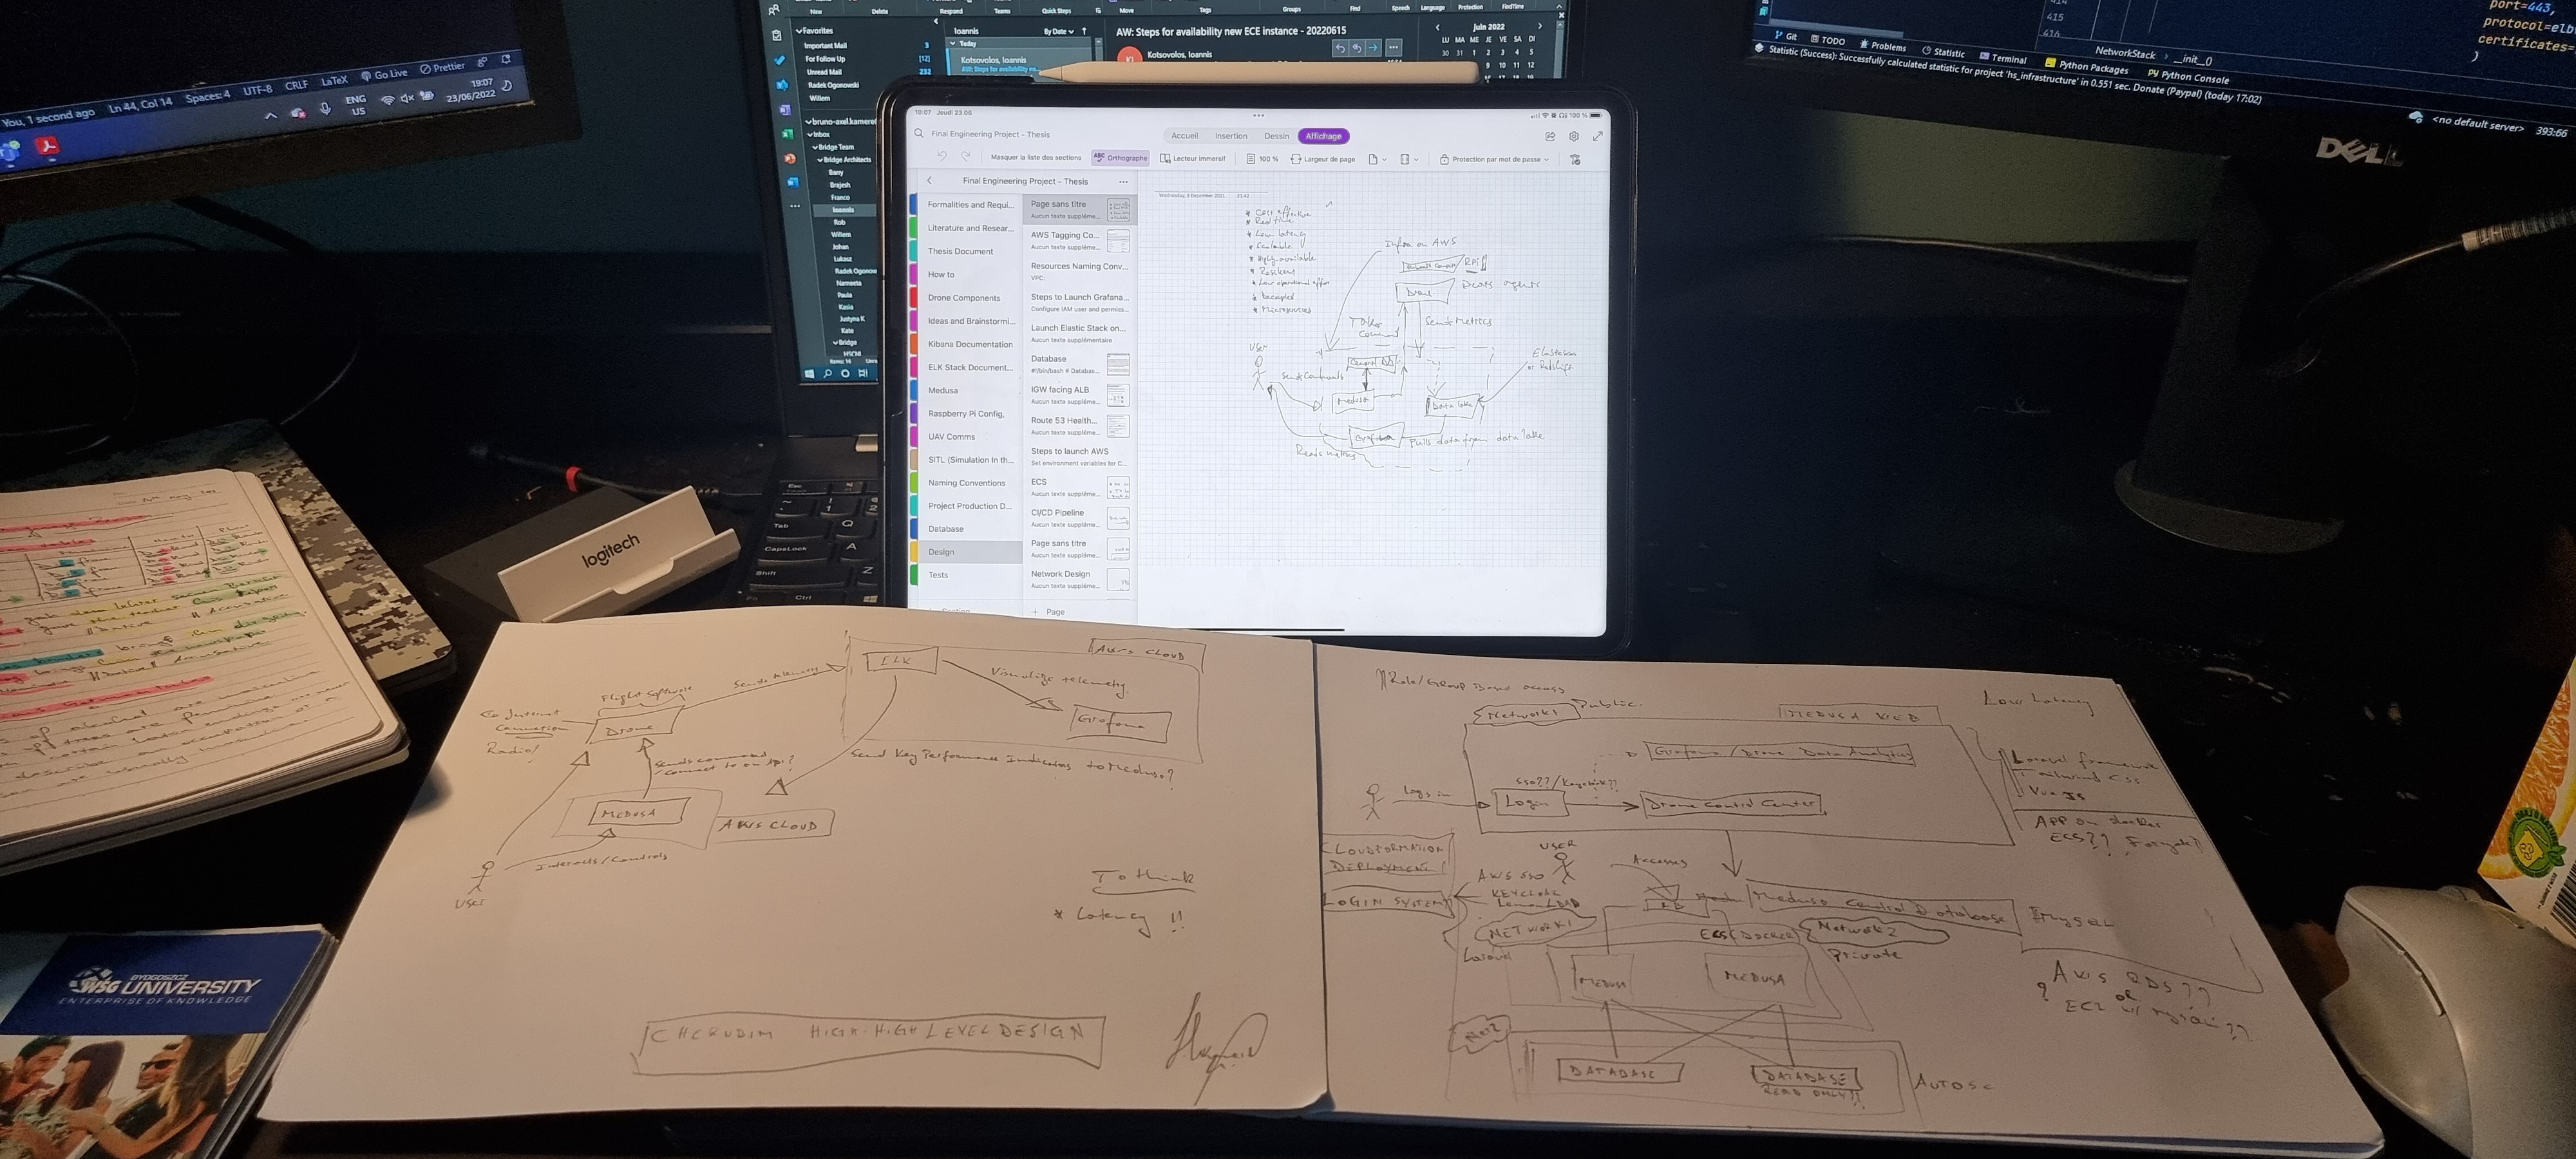
\includegraphics[width=1\linewidth]{initial_designs_2.jpg}
    \caption{Initial draft architecture designs.}
    \label{fig:initial-draft-designs}
    \source{Own work.}
\end{figure}

As the design started being built to reality, it was evident that deploying the whole AWS infrastructure manually from the AWS console, see figure \ref{fig:aws-console-home}, was going to be a time consuming and inefficient activity. And this also contradicted the initial idea of building an agile infrastructure that can be easily redeployed in case changes are needed. That is where the thought to build the infrastructure as code using some sort of infrastructure as code (IaC) tool came in. Since the cloud provider of choice was AWS, the best tool for the task was with no doubt the AWS' very own cloud development kit\cite{awscdkdocumentation}.

After the AWS infrastructure was built, the next step was the UAV. The outstanding questions here were:

\begin{itemize}
    \item How is the UAV going to be built?
    \item What is going to be the size?
    \item What is going to be the UAV type? Quadcopter? Fixed wing?
    \item How is the UAV going to be programmed? What programming language should be used?
    \item How is the UAV going to communicate with the rest of the system on AWS?
\end{itemize}

The above questions drove the next development stage. The UAV type of choice was a small quadcopter. The initial idea was to build an actual quadcopter, therefore the below parts were purchased to build the quadcopter from scratch:

\begin{itemize}
    \item Readytosky S500 quadcopter frame with built-in PCB.
    \item Pixhawk 2.4.8 flight controller with 4GB of onboard SD card storage.
    \item Raspberry Pi 4 model B with 4GB of onboard SD card storage.
    \item Readytosky M8N GPS module built-in compass with GPS antenna mount.
    \item 4 pieces of A2212 1000KV brushless motors.
    \item 4 pieces of 2-6S 30 amps Electronic speed controllers.
    \item 2 pairs of 1238 carbon fiber propellers.
\end{itemize}

<TODO: INSERT AN IMAGE OF THE ABOVE PARTS>

As the development of the quadcopter went on, it became obvious that this approach was not the best way to go, especially for a proof-of-concept (POC) solution mainly due to how costly it was becoming. At some point the wire connectors were even insufficient, and it came to notice that a power module was also needed, and it would take too long to order the parts online. The idea to build the actual physical quadcopter was then put on-hold, and it was decided to rather use simulation tools to simulate the actual quadcopter. Section \ref{sec:software-in-the-loop} elaborates more on how the simulation was implemented and set up.

%/--------------------------------- SECTION END ---------------------------------/%


%/-------------------------------- SECTION START --------------------------------/%

\section{Solution description}
\label{solution-description}

The proposed solution is a bit vast, here below the designs are going to be described and explained.

%/------------------------------ SUB-SECTION START ------------------------------/%

\subsection{AWS architecture high-level design}
\label{subsec:aws-architecture-hld}

One of the solution development best practice is to design first before attempting implementation. This helps one to brainstorm before hand how the solution to be built will look like. This approach was followed in developing the proposed solution. Figure \ref{fig:aws-architecture-hld} shows the high-level design that pictures a holistic view of how the AWS infrastructure looks like. It pictures how various AWS services talk to each other and how. The design is labeled with numbers, which are used to explain what each link is for in the following paragraph. Some of the components shown in design were not fully implemented but are part of the design as future work, that includes the continuous integration and continuous delivery (CI/CD) pipeline section on the left of the design, though it was tested separately and proven to work.

\begin{figure}[H]
    \centering 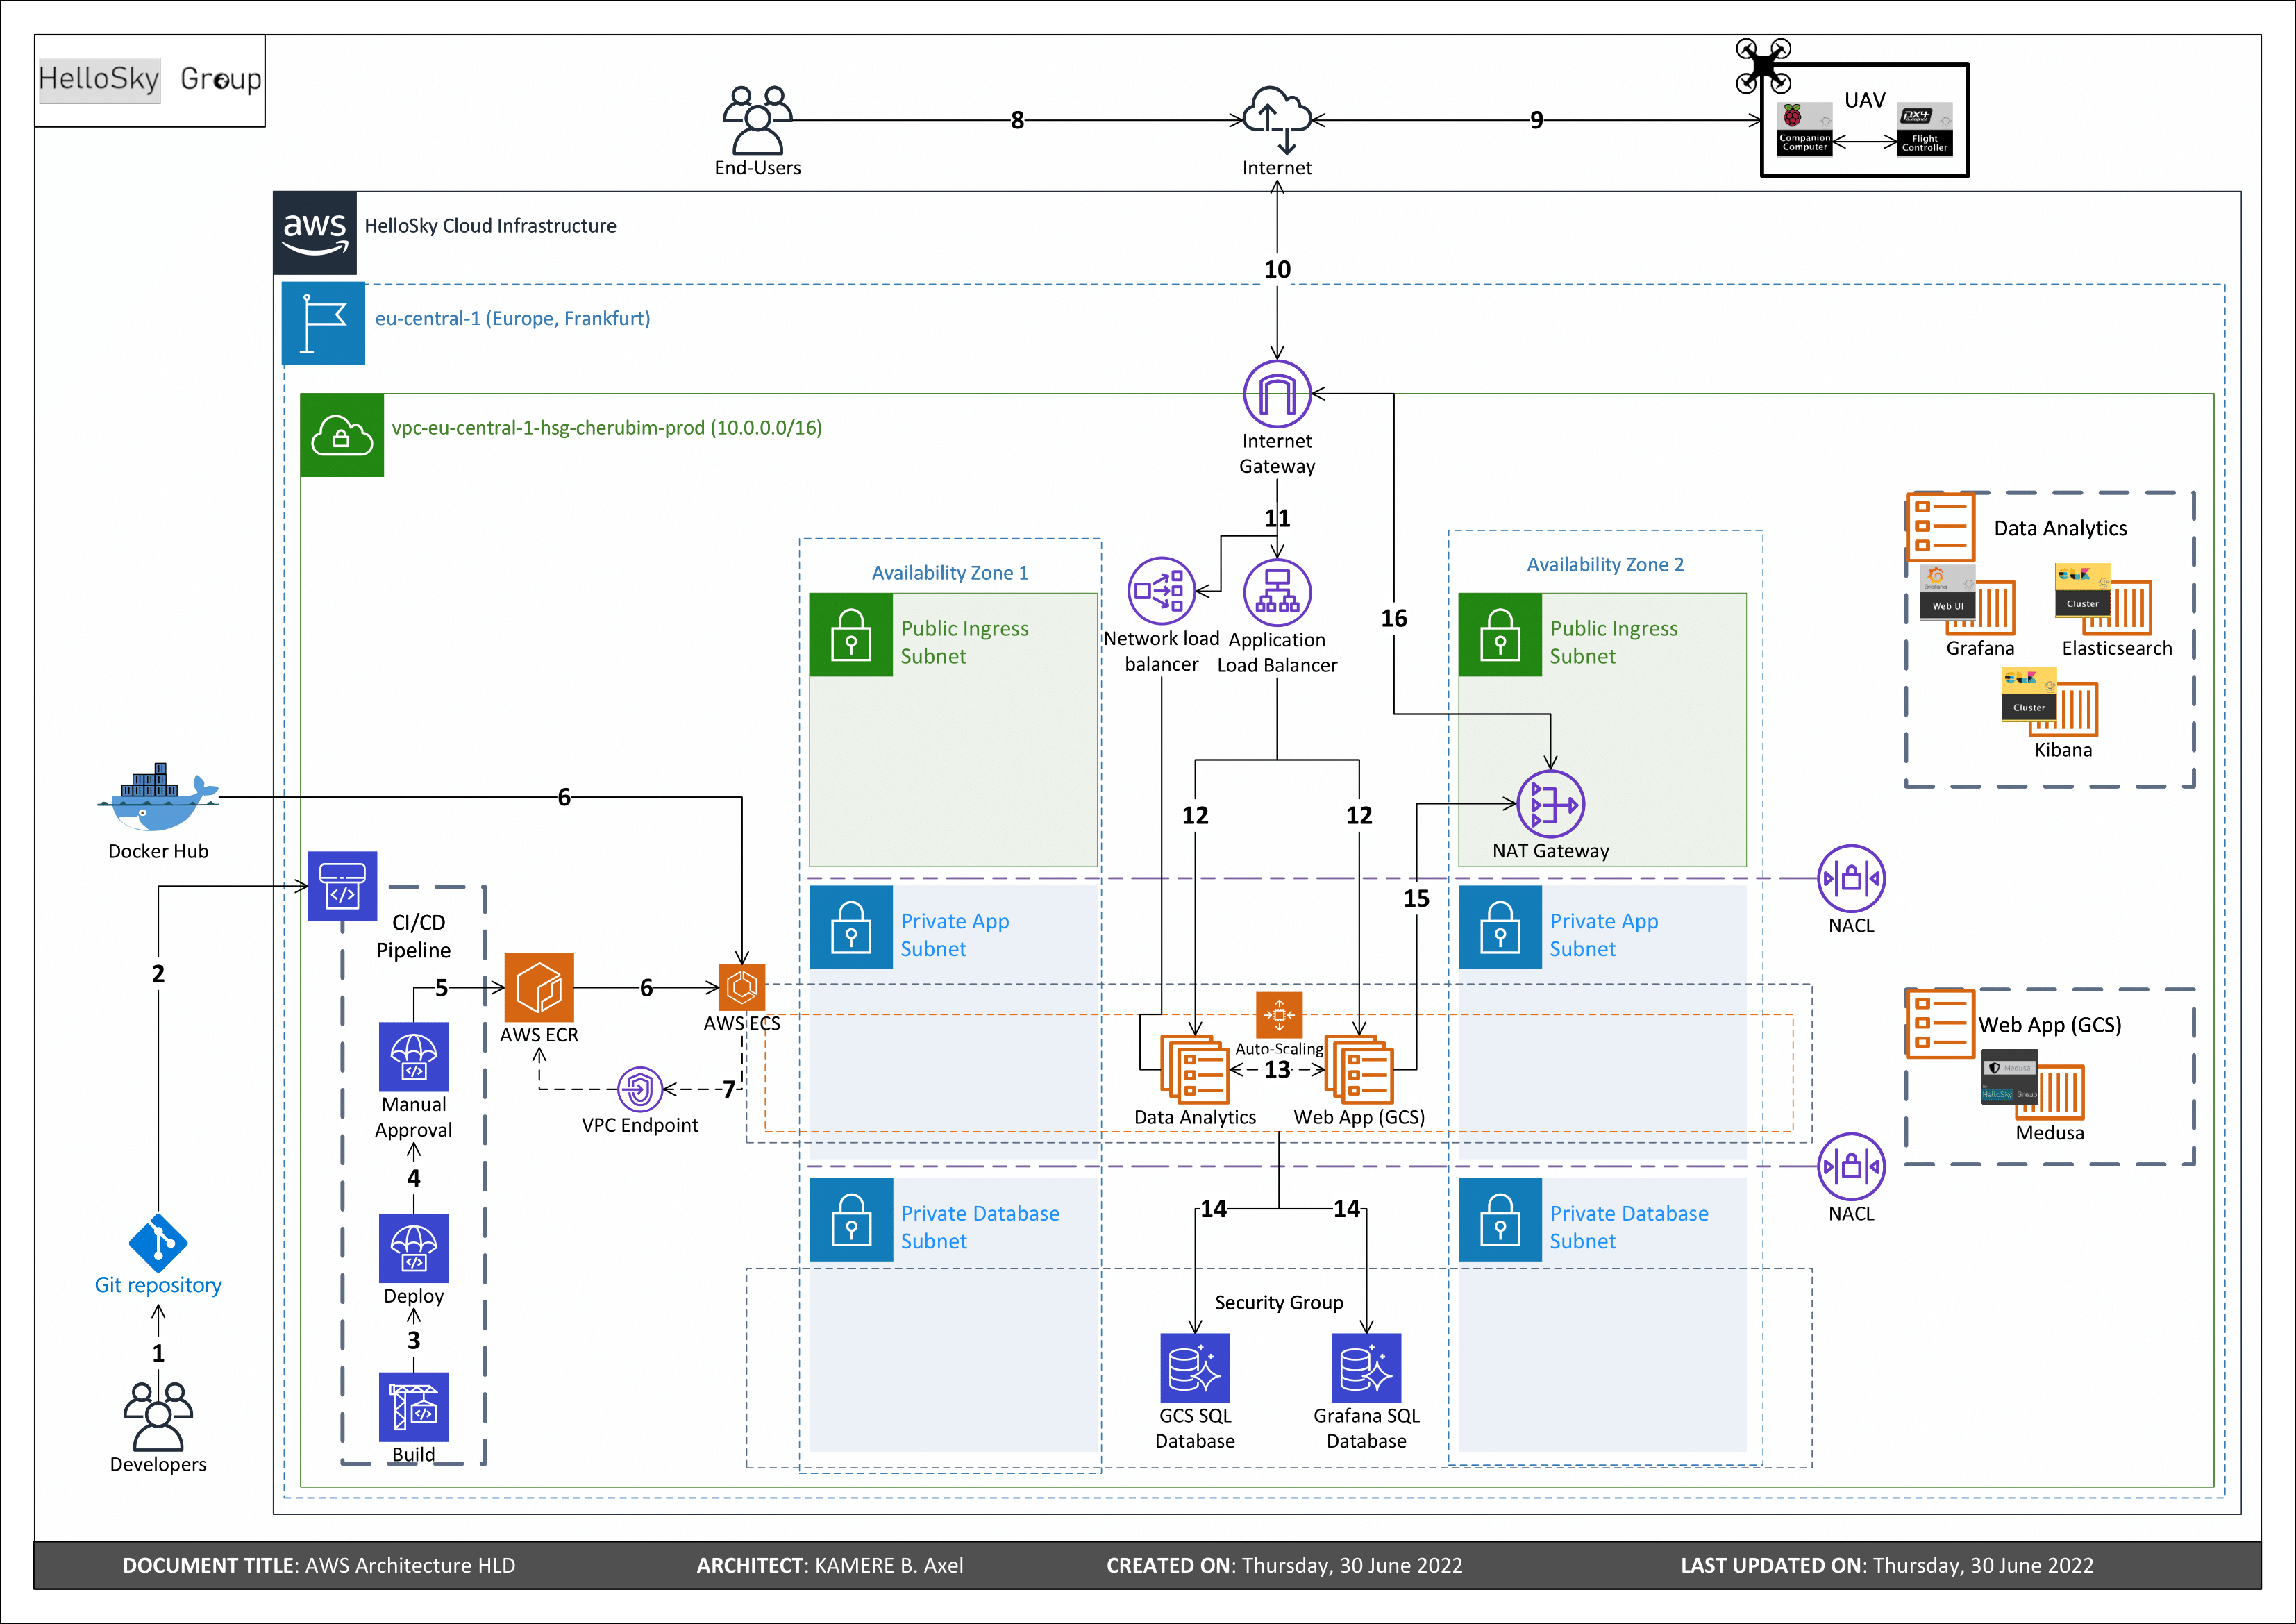
\includegraphics[width=1\linewidth]{aws_architecture_hld.png}
    \caption{Proposed AWS architecture high-level design.}
    \label{fig:aws-architecture-hld}
    \source{Own work. Designed with Microsoft Visio. Refer to \ref{subsec:ms-visio}.}
\end{figure}

Below are the explanations of the numbered items in the figure \ref{fig:aws-architecture-hld}:

Number 1 through 5 is a CI/CD pipeline that builds a docker image of the web app, the ground control station deployed on cloud.

\begin{enumerate}
    \item Developers commit code changes to a master branch of a Git repository.
    \item The activity triggers an AWS CloudWatch alarm, which then initiates the AWS CodePipeline.
    \item AWS CodeBuild service compiles the source code, runs tests and returns packaged application images ready to be deployed.
    \item After a package is created, the pipeline now waits for manual approval by an approver. This is so that only approved code are deployed to a production environment.
    \item Approved packaged images are pushed to the AWS Elastic Container Registry (ECR).
    \item Packages are pulled either from Docker Hub registry or from AWS ECR to build AWS containerised services.
    \item AWS Elastic Container Service (ECS) pulls images from AWS ECR via an AWS Virtual Private Cloud endpoint (VPC endpoint).
    \item Users can access front-end applications deployed on AWS through the internet
    \item The UAV sends telemetry to AWS services like the data lake and ground control station (GCS) and receives mission commands from the GCS via an LTE or WiFi data link.
    \item All traffic that go to an AWS VPC have to go through an internet gateway. Without it, AWS VPC resources cannot talk to the internet.
    \item All incoming traffic is load balanced with an AWS application load balancer (AWS ALB) which will then forward the traffic to desired services depending on the requested resource.
    \item Traffic is routed to the desired target group configured on the AWS ALB.
    \item The GCS and data analytics services like the telemetry dashboards and the data lake can communicate to each other.
    \item Grafana that runs the telemetry dashboards has a MySQL database that the Grafana service can access in the private isolated subnet. Same goes for the GCS.
    \item Resources deployed in private have no direct communication with the internet, therefore for them to pull updates, a network address translation gateway (NAT gateway) is needed to establish the connection.
    \item The NAT gateway the goes through the internet gateway then to the internet.
\end{enumerate}

%/------------------------------- SUB-SECTION END -------------------------------/%


%/------------------------------ SUB-SECTION START ------------------------------/%

\subsection{AWS cloud development kit setup}
\label{subsec:aws-cdk-setup}

The AWS infrastructure described in section \ref{subsec:aws-architecture-hld} is deployed as code using AWS cloud development kit (AWS CDK). AWS CDK allows developers to build AWS infrastructures in an agile manner by using normal programming languages. This allows developers to take advantage of programming idioms like loops, variables, conditionals and inheritance to build robust AWS infrastructures. This also means that software engineering practices like source control, testing and code reviews can be used since the infrastructure is basically standard code. Currently AWS CDK supports Python, Javascript, C\#, Go, and Typescript programming languages.

A typical AWS CDK project is made up of 3 components, namely:

\begin{itemize}
    \item an app. This is the overall set of everything. An AWS CDK project is basically called an AWS CDK app. This comprises of constructs.
    \item constructs. These represent components that make an AWS infrastructure. They can be an AWS simple storage service (S3), an elastic cloud compute (EC2), an application load balancer (ALB) \textit{et cetera}. AWS has a comprehensive site that shows all the available AWS and community constructs\cite{awsconstructhub}.
    \item stacks. These are the unit of deployment in AWS CDK. A stack represents all AWS resources defined within the same scope.
\end{itemize}

Figure \ref{fig:aws-cdk-app-structure} shows how an AWS CDK app is structured.

\begin{figure}[H]
    \centering 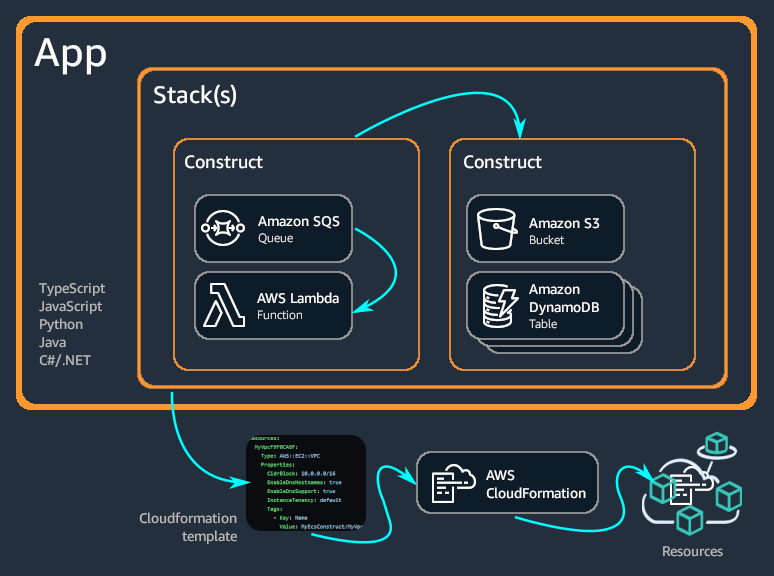
\includegraphics[width=1\linewidth]{aws_cdk_workflow.png}
    \caption{AWS CDK app structure.}
    \label{fig:aws-cdk-app-structure}
    \source{AWS CDK documentation\cite{awscdkdocumentation}.}
\end{figure}

%/------------------------------- SUB-SECTION END -------------------------------/%


%/------------------------------ SUB-SECTION START ------------------------------/%

\subsection*{Build}
\label{subsec:build}

To start building the AWS infrastructure with AWS CDK, the AWS command line interface (CLI) needs to first be set up. To install the AWS CLI on Windows, run the following command \mintinline[breaklines, breakanywhere]{bash}{msiexec.exe /i https://awscli.amazonaws.com/AWSCLIV2.msi}. This allows to interact with AWS via the CLI.

Once the AWS CLI is installed, type the command \mintinline[breaklines, breakanywhere]{bash}{aws configure} to configure credentials to AWS. The console will ask for the AWS access key ID, the AWS secret access key, the default region name and the default output format as shown in figure \ref{fig:aws-configure-output}.

\begin{figure}[H]
    \centering 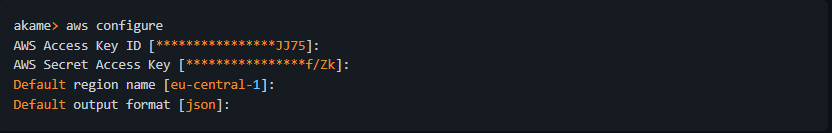
\includegraphics[width=1\linewidth]{aws_configure_output.png}
    \caption{AWS configure CLI output.}
    \label{fig:aws-configure-output}
    \source{Own work.}
\end{figure}

The next step is to then install AWS CDK from node package manager (NPM) with \mintinline[breaklines, breakanywhere]{bash}{npm install -g aws-cdk}. This will download and install the latest aws-cdk version on the local workstation. The "-g" flag makes the package available globally on the workstation.

Next, get the account number from the AWS CLI using the AWS security token service (STS) and the region name from AWS CLI configuration by executing the commands below.

\mintinline[breaklines, breakanywhere]{bash}{aws sts get-caller-identity}, to get the account number.

\mintinline[breaklines, breakanywhere]{bash}{aws configure get region}, to get the region name.

\begin{figure}[H]
    \centering 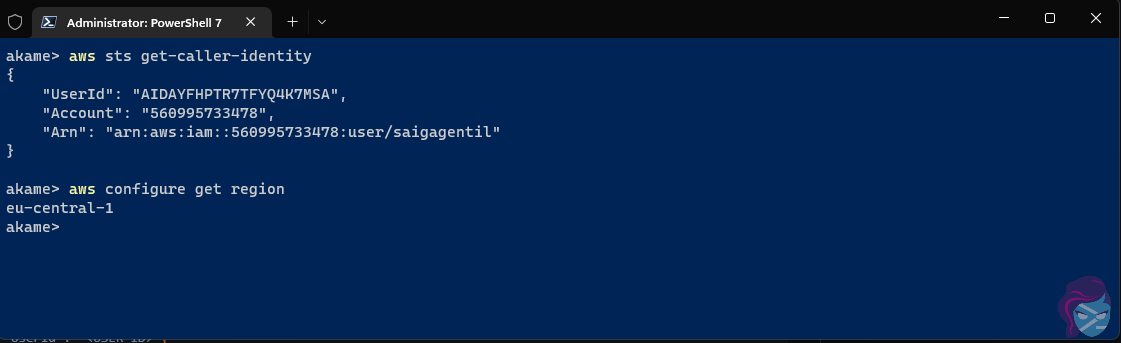
\includegraphics[width=1\linewidth]{cdk_pre_bootstrap.png}
    \caption{AWS STS and configure commands output.}
    \label{fig:aws-account-numbre-region}
    \source{Own work.}
\end{figure}

With the account number and the region name, AWS CDK can be bootstrapped now. Bootstrapping in AWS refers to the process of creating assets (local files, directories, docker image,...) that need to be deployed with the stack. These assets are deployed to an AWS S3 bucket for AWS CloudFormation to use them during stack deployment. Execute command \mintinline[breaklines, breakanywhere]{bash}{cdk bootstrap aws://560995733478/eu-central-1} to bootstrap AWS CDK.

Once all the above steps are completed, a CDK app can now be created. First create a directory for the app and move into the directory, \mintinline[breaklines, breakanywhere]{bash}{mkdir hs_infrastructure} then \mintinline[breaklines, breakanywhere]{bash}{cd hs_infrastructure},then run the command \mintinline[breaklines, breakanywhere]{bash}{cdk init app --language python} to initialize a Python AWS CDK app. After that, activate the Python virtual environment with \mintinline[breaklines, breakanywhere]{bash}{source .venv/Scripts/activate} and install the core AWS CDK plugins with \mintinline[breaklines, breakanywhere]{bash}{python -m pip install -r requirements.txt}.

This will generate a couple of starting files in the app directory. Also if Git is installed on the workstation the app will be initialized as a Git repository that can be versioned and later be pushed to a Git remote repository like Github.

%/------------------------------- SUB-SECTION END -------------------------------/%


%/------------------------------ SUB-SECTION START ------------------------------/%

\subsection*{Deploy}
\label{subsec:deploy}

After completing the previous steps, we have an app with a default stack but with no resources defined in it. The next step is to write code that defines stacks that make the AWS infrastructure. In the proposed solution, multiple stacks were created, figure \ref{fig:aws-stacks} shows the stacks that make the proposed solution.

\begin{figure}[H]
    \centering 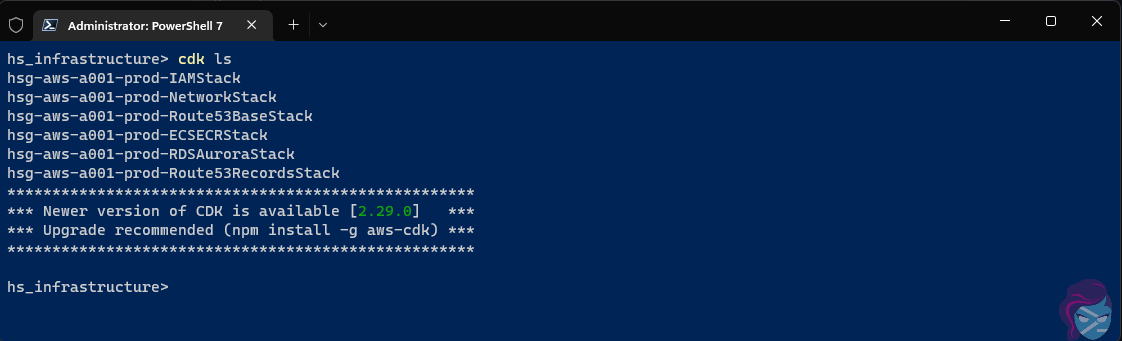
\includegraphics[width=1\linewidth]{cdk_ls.png}
    \caption{Proposed solution AWS stacks.}
    \label{fig:aws-stacks}
    \source{Own work.}
\end{figure}

Each of the stacks defines several services needed to build the whole overall infrastructure.
\begin{itemize}
    \item hsg-aws-a001-prod-IAMStack: Creates IAM user needed by the AWS elastic container service (ECS) and elastic container registry (ECR).
    \item hsg-aws-a001-prod-NetworkStack: Sets up the overall AWS infrastructure networking. Subnets, firewall rules, \textit{et cetera}. This is the longest stack in terms of lines of code, because it is made up of approximately 480 lines of code.
    \item hsg-aws-a001-prod-Route53BaseStack: This creates a hosted zone for the domain helloskygroup.com as well as a wildcard SSL certificate for the domain.
    \item hsg-aws-a001-prod-ECSECRStack: This spins up docker containers hosting the web application in the AWS ECS Fargate service. Fargate was used since it is a serverless service. A serverless service is a service that offloads the responsibility from developers to managed the actual physical servers hosting the deployed resources.
    \item hsg-aws-a001-prod-RDSAuroraStack: This deploys a MySQL database in the AWS relational database service (RDS).
    \item hsg-aws-a001-prod-Route53RecordsStack: This adds DNS records in the hosted zone created in the 'hsg-aws-a001-prod-Route53BaseStack' stack.
\end{itemize}

Once each stack is developed, the next step is to deploy it to AWS. Snippet \ref{code:hs_infrastructure_app_snippet_1} shows the \mintinline[breaklines, breakanywhere]{python}{main.py} code that basically imports all the created tasks in the AWS app and executes them. From there, the command \mintinline[breaklines, breakanywhere]{bash}{cdk deploy -all} needs to be executed from the root directory to deploy the resources and stacks defined in the app. Figure \ref{fig:aws-cdk-app-lifecycle} shows the full lifecycle of an AWS CDK app.

\begin{figure}[H]
    \centering 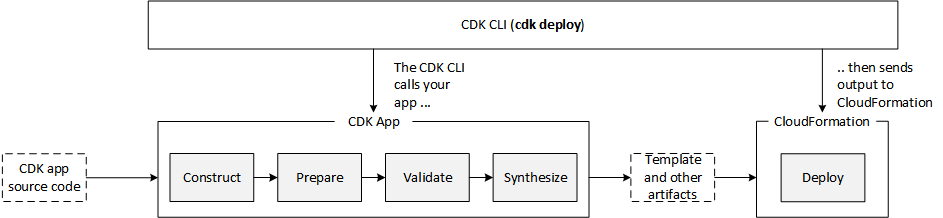
\includegraphics[width=1\linewidth]{aws_cdk_app_lifecycle.png}
    \caption{AWS CDK app lifecycle.}
    \label{fig:aws-cdk-app-lifecycle}
    \source{AWS documentation\cite{awscdkdocumentationapps}.}
\end{figure}

\begin{center}
    \captionsetup{type=listing}
    \inputminted[
        frame=single,
        framesep=2mm,
        baselinestretch=1.2,
        fontsize=\footnotesize,
        breaklines,
        breakanywhere,
        linenos
    ]{python}{config/code/47c895ea0838ad6366c2b0e53bb8c331/hs_infrastructure_app_snippet_1.py}
    \captionof{listing}{AWS CDK app.py snippet.}
    \label{code:hs_infrastructure_app_snippet_1}
\end{center}

%/--------------------------------- SECTION END ---------------------------------/%


%/-------------------------------- SECTION START --------------------------------/%

\section{AWS network and security configuration}
\label{sec:aws-network}

One of the challenges with implementing a networked system, especially on cloud platforms like AWS, is ensuring that traffic flows in the expected way with proper security in place. The proposed solution, being a networked solution involving communications to and from various applications, has a rigorous network design. Figure \ref{fig:aws-network-hld} shows how network within the proposed AWS infrastructure was designed.

AWS' Virtual Private Cloud also known as VPC concept, which is simply an isolated private network on the cloud. The VPC in the proposed solution is configured with network range 10.0.0.0/16 which is broken down in 3 subnets for each of the two availability zones that make the eu-central-1 (Frankfurt) region in which the AWS resources are deployed in.


%/------------------------------ SUB-SECTION START ------------------------------/%

\subsubsection*{eu-central-1a availability zone}
\label{eu-central-1a-az}

\begin{itemize}
    \item Public subnet. Configured with network range 10.0.0.0/24.
    \item Private subnet. Configured with network range 10.0.2.0/24.
    \item Private-isolated subnet. Configured with network range 10.0.4.0/28.
\end{itemize}

%/------------------------------- SUB-SECTION END -------------------------------/%


%/------------------------------ SUB-SECTION START ------------------------------/%

\subsubsection*{eu-central-1b availability zone}
\label{eu-central-1b-az}

\begin{itemize}
    \item Public subnet. Configured with network range 10.0.1.0/24.
    \item Private subnet. Configured with network range 10.0.3.0/24.
    \item Private-isolated subnet. Configured with network range 10.0.4.16/28.
\end{itemize}

\begin{figure}[H]
    \centering 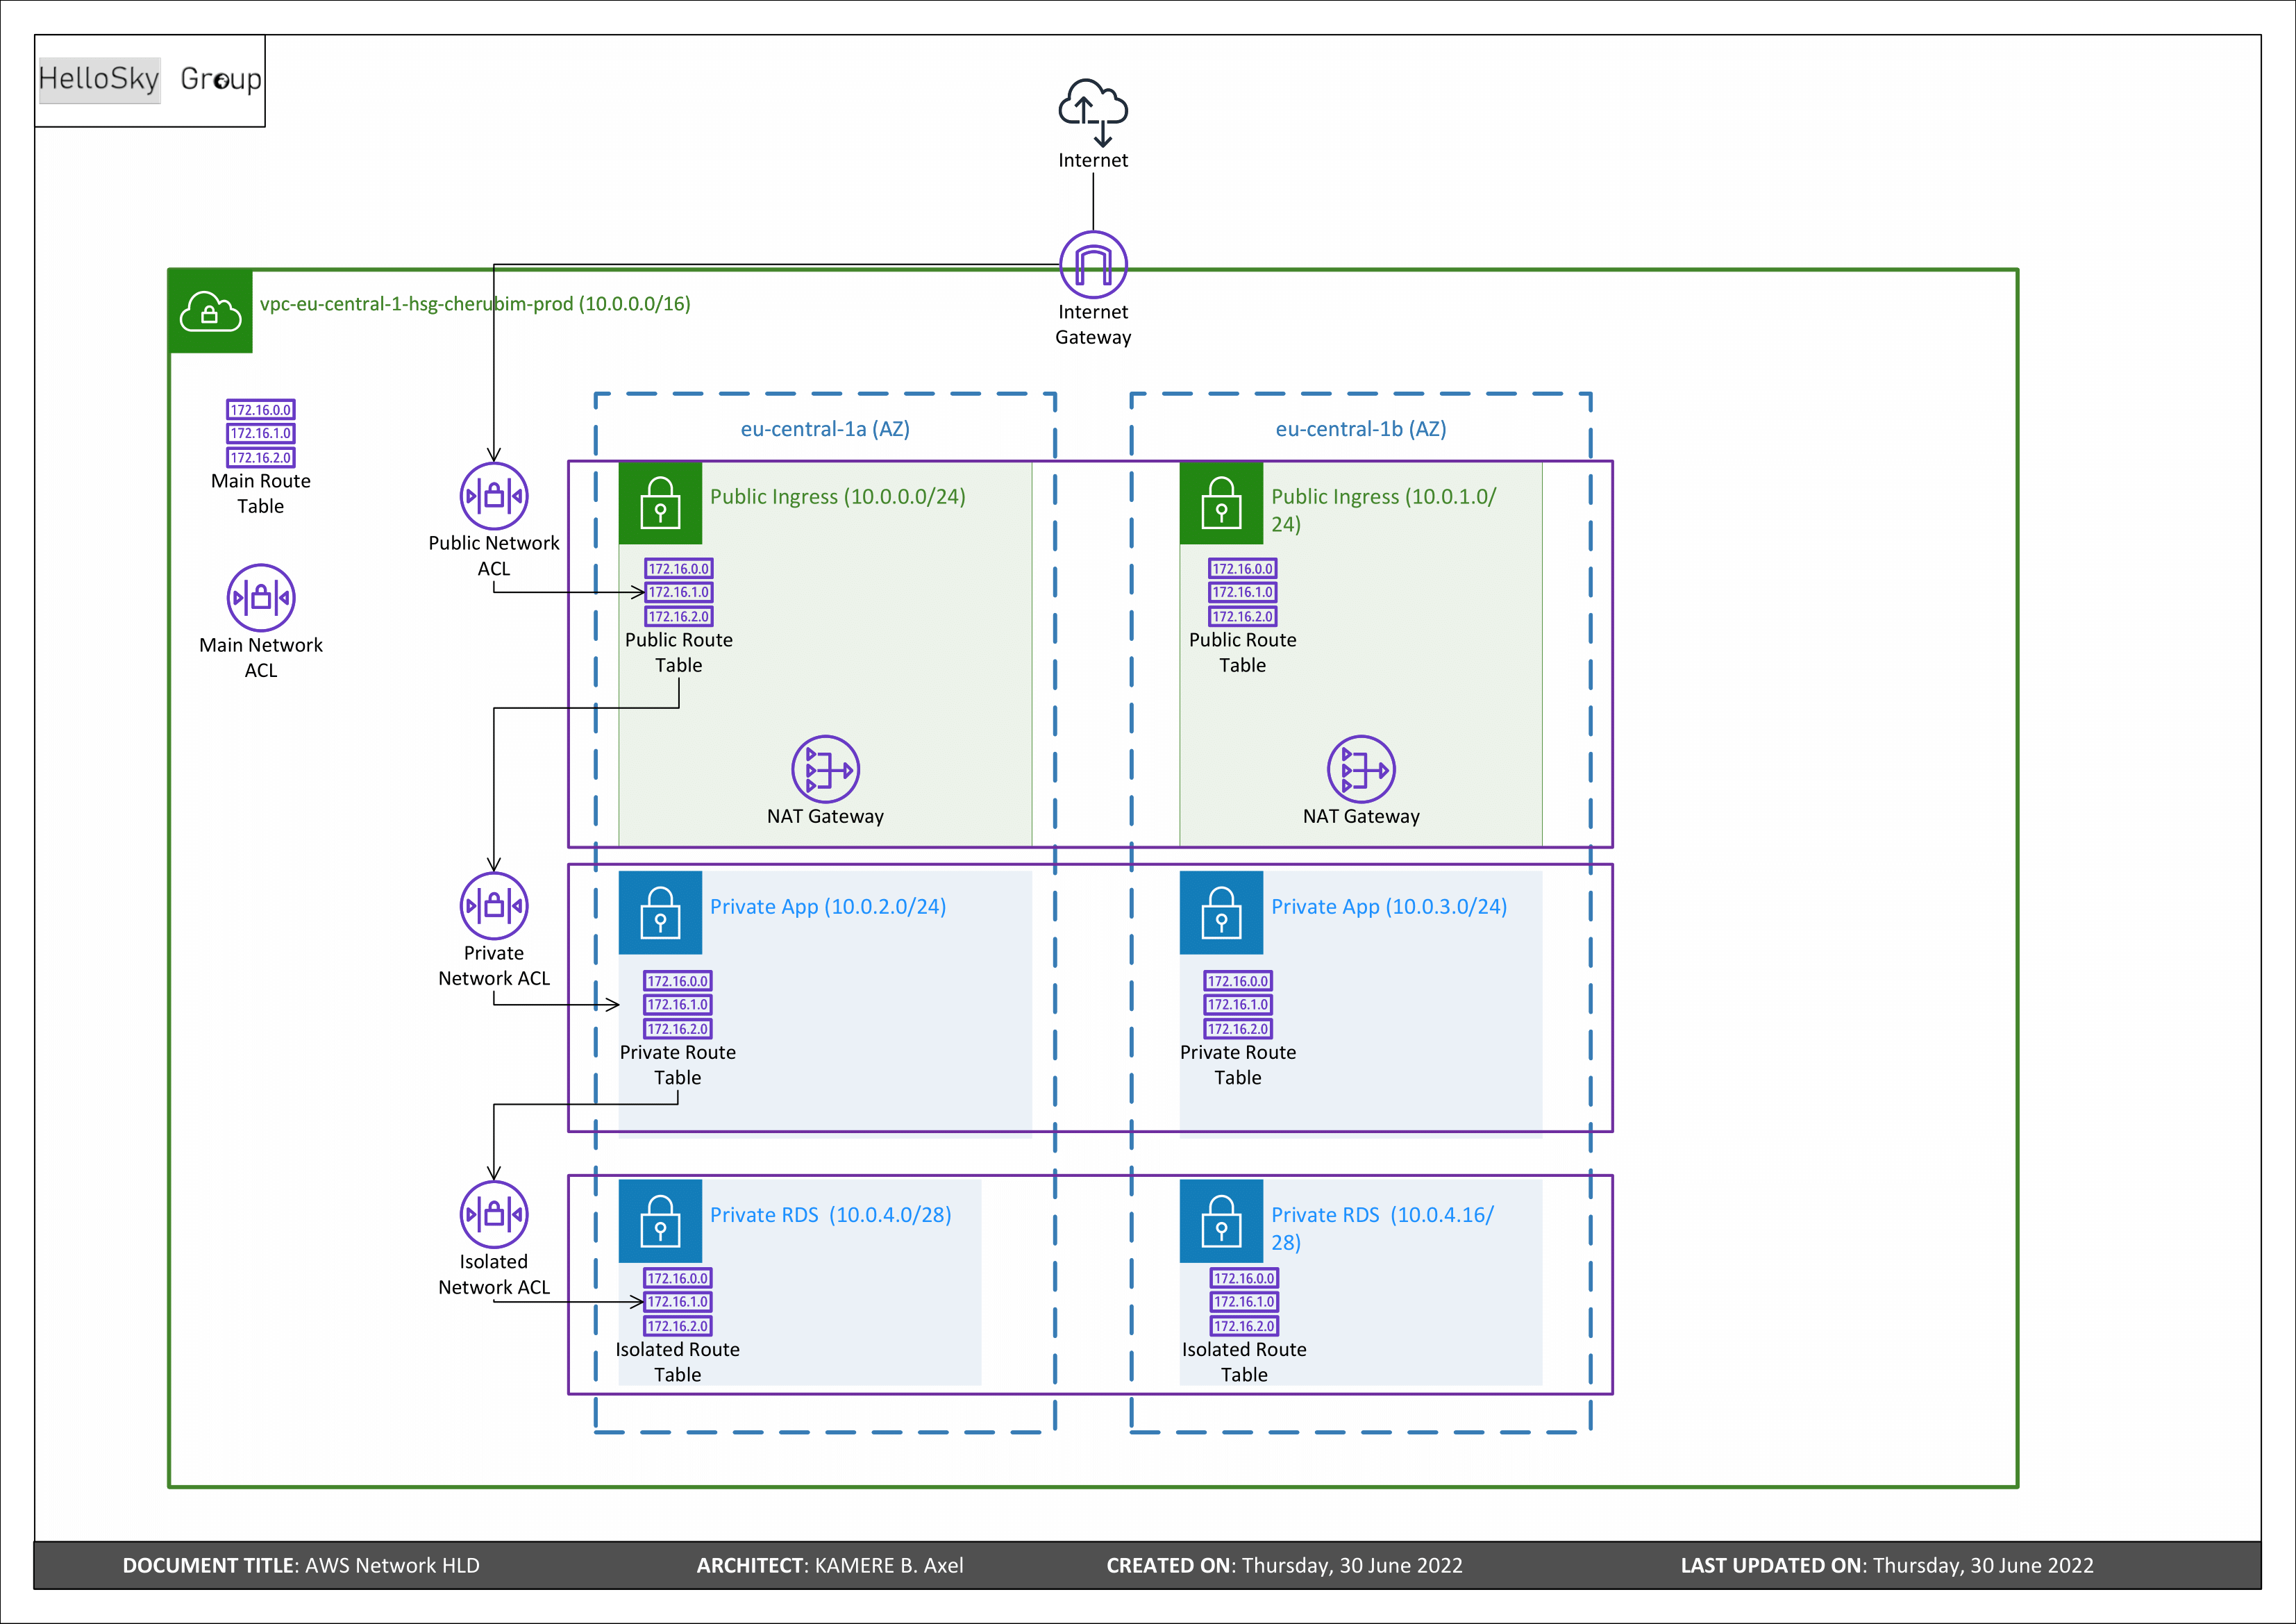
\includegraphics[width=1\linewidth]{aws_network_hld.png}
    \caption{AWS network high-level design.}
    \label{fig:aws-network-hld}
    \source{Own work. Designed with Microsoft Visio. Refer to \ref{subsec:ms-visio}.}
\end{figure}

%/------------------------------- SUB-SECTION END -------------------------------/%


%/------------------------------ SUB-SECTION START ------------------------------/%

\subsection{Public subnet}
\label{public-subnet}

The public subnet in this proposed solution does not contain any resources, except a Network Address Translation or NAT gateway that is used by resources in the private subnet to access the internet. Table \ref{table:public-subnet-inbound} and \ref{table:public-subnet-outbound} show the inbound and outbound traffic rules respectively configured on the public subnet network access control list or NACL.

\begin{table}[H]
    \centering
    \begin{tabular}{|c|c|c|c|c|c|}
        \hline
        \multicolumn{6}{|c|}{Inbound traffic}                               \\
        \hline
        Rule & Type        & Protocol & Port range & Source    & Allow/Deny \\
        \hline
        100  & HTTP (80)   & TCP (6)  & 80         & 0.0.0.0/0 & Allow      \\
        \hline
        110  & HTTPS (443) & TCP (6)  & 443        & 0.0.0.0/0 & Allow      \\
        \hline
        120  & Custom TCP  & TCP (6)  & 1024-65535 & 0.0.0.0/0 & Allow      \\
        \hline
        *    & All IPV4    & All      & All        & 0.0.0.0/0 & Deny       \\
        \hline
    \end{tabular}
    \caption{Public subnet NACL inbound traffic rules}
    \label{table:public-subnet-inbound}
\end{table}

\begin{itemize}
    \item \textbf{Rule 100:} Allows inbound HTTP traffic on port 80 towards any IPv4 address on the internet.
    \item \textbf{Rule 110:} Allows inbound HTTPS traffic on port 443 towards any IPv4 address on the internet.
    \item \textbf{Rule 120:} Allows returning TCP traffic from the internet responding to requests from the subnet. The specified port ranges are ephemeral ports as defined by the Internet Assigned Number Authority or IANA and Internet Engineering Task Force or IETF in their Request for Comments or RFC 6056 document \cite{rfc6056}.
    \item \textbf{Rule *:} Block every other non previously evaluated IPv4 traffic.
\end{itemize}

\begin{table}[H]
    \centering
    \begin{tabular}{|c|c|c|c|c|c|}
        \hline
        \multicolumn{6}{|c|}{Outbound traffic}                                \\
        \hline
        Rule & Type        & Protocol & Port range & Destination & Allow/Deny \\
        \hline
        100  & HTTP (80)   & TCP (6)  & 80         & 0.0.0.0/0   & Allow      \\
        \hline
        110  & HTTPS (443) & TCP (6)  & 443        & 0.0.0.0/0   & Allow      \\
        \hline
        120  & Custom TCP  & TCP (6)  & 1024-65535 & 0.0.0.0/0   & Allow      \\
        \hline
        *    & All IPV4    & All      & All        & 0.0.0.0/0   & Deny       \\
        \hline
    \end{tabular}
    \caption{Public subnet NACL outbound traffic rules}
    \label{table:public-subnet-outbound}
\end{table}

The rules explanation are similar to those for inbound traffic in table \ref{table:public-subnet-inbound}, except that instead of inbound it is outbound.

%/------------------------------- SUB-SECTION END -------------------------------/%


%/------------------------------ SUB-SECTION START ------------------------------/%

\subsection{Private subnet}
\label{private-subnet}

Most of the infrastructure components are deployed in the private subnet where only specific traffic from the public and isolated-private subnets are allowed in. In this subnet is where the UAV command and control center user interface is deployed, in containers using the AWS Fargate serverless service. The rules for this subnet have to be carefully defined so that;

\begin{itemize}
    \item Fargate services can pull docker images from docker hub public repositories on the internet.
    \item The UAV, and several command and control application services can talk to each other.
\end{itemize}

Table \ref{table:private-subnet-inbound} and \ref{table:private-subnet-outbound} show the inbound and outbound traffic rules respectively configured on the private subnet network access control list or NACL.

\begin{table}[H]
    \centering
    \begin{tabular}{|c|c|c|c|c|c|}
        \hline
        \multicolumn{6}{|c|}{Inbound traffic}                                 \\
        \hline
        Rule & Type        & Protocol & Port range & Source      & Allow/Deny \\
        \hline
        100  & HTTP (80)   & TCP (6)  & 80         & 0.0.0.0/0   & Allow      \\
        \hline
        110  & HTTPS (443) & TCP (6)  & 443        & 0.0.0.0/0   & Allow      \\
        \hline
        120  & Custom TCP  & TCP (6)  & 1024-65535 & 0.0.0.0/0   & Allow      \\
        \hline
        130  & Custom TCP  & TCP (6)  & 3306       & 10.0.4.0/28 & Allow      \\
        \hline
        140  & Custom TCP  & TCP (6)  & 3306       & 10.0.5.0/28 & Allow      \\
        \hline
        *    & All IPV4    & All      & All        & 0.0.0.0/0   & Deny       \\
        \hline
    \end{tabular}
    \caption{Private subnet NACL inbound traffic rules}
    \label{table:private-subnet-inbound}
\end{table}

\begin{itemize}
    \item \textbf{Rule 100:} Allows inbound HTTP traffic on port 80. This is so that the AWS Elastic Container Service or ECS tasks can pull images from the public Dockerhub registry.
    \item \textbf{Rule 110:} Allows inbound HTTPS traffic on port 443.
    \item \textbf{Rule 120:} Allows returning TCP traffic from the internet responding to requests from the subnet.
    \item \textbf{Rule 130 and Rule 140:} Allows inbound traffic on port 3306 from MySQL database running in the AWS Relational Database Service or AWS within the isolated-private subnets of both the Availability Zones.
    \item \textbf{Rule *:} Blocks every other non previously evaluated IPv4 traffic.
\end{itemize}

\begin{table}[H]
    \centering
    \begin{tabular}{|c|c|c|c|c|c|}
        \hline
        \multicolumn{6}{|c|}{Outbound traffic}                                \\
        \hline
        Rule & Type        & Protocol & Port range & Destination & Allow/Deny \\
        \hline
        100  & HTTP (80)   & TCP (6)  & 80         & 0.0.0.0/0   & Allow      \\
        \hline
        110  & HTTPS (443) & TCP (6)  & 443        & 0.0.0.0/0   & Allow      \\
        \hline
        120  & Custom TCP  & TCP (6)  & 1024-65535 & 0.0.0.0/0   & Allow      \\
        \hline
        130  & Custom TCP  & TCP (6)  & 3306       & 10.0.4.0/28 & Allow      \\
        \hline
        140  & Custom TCP  & TCP (6)  & 3306       & 10.0.5.0/28 & Allow      \\
        \hline
        *    & All IPV4    & All      & All        & 0.0.0.0/0   & Deny       \\
        \hline
    \end{tabular}
    \caption{Private subnet NACL outbound traffic rules}
    \label{table:private-subnet-outbound}
\end{table}

\begin{itemize}
    \item \textbf{Rule 100:} Allows outbound HTTP traffic on port 80 towards any IPv4 address.
    \item \textbf{Rule 110:} Allows outbound HTTPS traffic on port 443 towards any IPv4 address.
    \item \textbf{Rule 120:} Allows all outbound response TCP traffic.
    \item \textbf{Rule *:} Blocks every other non previously evaluated IPv4 traffic.
\end{itemize}

<TALK ABOUT SECURITY GROUPS>

%/------------------------------- SUB-SECTION END -------------------------------/%


%/------------------------------ SUB-SECTION START ------------------------------/%

\subsection{Isolated-private subnet}
\label{isolated-private-subnet}

The isolated-private subnet hosts the MySQL database running in AWS Relational Database Service. This subnet only talks to the private subnet, and has no direct connection to the internet. This improves the infrastructure security through not exposing the database directly to the internet.

<ADD NETWORK FLOW DESIGNS>

Describe the solution on a higher level. Discuss HLDs.

%/--------------------------------- SECTION END ---------------------------------/%


%/-------------------------------- SECTION START --------------------------------/%

\section{Software in the loop UAV simulator}
\label{sec:software-in-the-loop}

%/--------------------------------- SECTION END ---------------------------------/%


%/-------------------------------- SECTION START --------------------------------/%

\section{UAV Communication}
<Talk about Mavlink... and how mavlink is used in the project>

%/--------------------------------- SECTION END ---------------------------------/%

%/--------------------------------- CHAPTER END ---------------------------------/%


%/----------------------------- NOMENCLATURE START ------------------------------/%

\nomenclature[z-AZ]{AZ}{Availability Zone}
\nomenclature[z-NAT]{NAT}{Network Address Translation}
\nomenclature[z-VPC]{VPC}{Virtual Private Cloud}
\nomenclature[z-HTTP]{HTTP}{Hypertext Transfer Protocol}
\nomenclature[z-HTTPS]{HTTPS}{Hypertext Transfer Protocol Secured}
\nomenclature[z-ECS]{ECS}{Elastic Container Service}
\nomenclature[z-NACL]{NACL}{Network Access Control List}
\nomenclature[z-EC2]{EC2}{Elastic Cloud Compute}
\nomenclature[z-TCP]{TCP}{Transmisison Control Protocol}
\nomenclature[z-RDS]{RDS}{Relational Database Service}
\nomenclature[z-ALB]{ALB}{Application Load Balancer}
\nomenclature[z-RDS]{RDS}{Relational Database Service}
\nomenclature[z-IANA]{IANA}{Internet Assigned Number Authority}
\nomenclature[z-IETF]{IETF}{Internet Engineering Task Force}
\nomenclature[z-RFC]{RFC}{Request for Comments}
\nomenclature[z-PCB]{PCB}{Printed Circuit Board}
\nomenclature[z-SD]{SD (as in SD card)}{Secure Digital}
\nomenclature[z-GPS]{GPS}{Global Positioning System}
\nomenclature[z-S3]{S3 (as in AWS S3)}{Simple Storage Service}
\nomenclature[z-CLI]{CLI}{Command Line Interface}
\nomenclature[z-IAM]{IAM}{Identity Access Management}
\nomenclature[z-ECR]{ECR}{Elastic Container Registry}

%/------------------------------ NOMENCLATURE END -------------------------------/%


%--------------------------------
% Chapters - Setup
%--------------------------------
% \cleardoublepage
% % ------------------------------------------------------------------------
% 60. Setup
% ------------------------------------------------------------------------

\chapter{Setup}


%---------------------------------4.1 Software---------------------------------%
\section{Software}

% Command and Control Center Portal (Medusa)
\subsection{Command and Control Center Portal}

% Command and Control Center Portal (Medusa)
\subsection{Telemetry dashboard}

%---------------------------------4.2 Hardware---------------------------------%
\section{Hardware}




%--------------------------------
% Chapters - Discussion
%--------------------------------
% ------------------------------------------------------------------------
% 70. Discussion
% ------------------------------------------------------------------------

\chapter{Discussion}
\label{chap:discussion}

Designing, deploying and implementing a robust and scalable unmanned aerial system running on the cloud can be a challenging task given how many components involved that have to talk to each other in the system. Making sure that all components talk has been one of the main challenges during the project implementation.

The cloud component part has specifically posed quite a challenge to make sure that all the components can talk, ensuring that proper firewall and traffic rules are set was not easy at first, until the whole VPC traffic log started being captured and analysed. VPC flow log, an AWS network logging feature that logs all traffic flowing through all network interfaces throughout the VPC, was used to analyse the traffic. The logs would expose how traffic would flow and would indicate where traffic was being blocked. This helped then with the design of the firewall rules.

<To-do: Attach a screenshot of VPC flow log traffic>

Other than the networking aspect on AWS, integrating the UAV itself  was also quite challenging. As mentioned throughout this document, the initial idea was to build the solution with physical UAV parts. They were even available, but some parts were missing and due to how difficult it was to find them on the market, in a sense that they had to be ordered from places like China and would take some time to be delivered, it became a blocker to progress the project with actual UAV hardware. The UAV was then simulated, as described in section \ref{sec:simulation}. Simulating the UAV was not that much of a big challenge due to the very good documentation available.

Despite all the challenges faced, the use of the cloud in the unmanned aerial mobility sector seemed to be an area that can revolutionize and significantly contribute in the development of the sector. The use of various deployment techniques like infrastructure as code as described in section \ref{subsec:aws-cdk-setup} can also help in speeding up infrastructure deployment times, making the infrastructure agile and facilitating maintenance.

Making UAVs systems easy to deploy increases their accessibility to civilians thus improving several use case processes like agriculture irrigation, disaster management, \textit{et cetera}. Even though, making UAVs accessible to the public would bring positive outcomes, it would also bring a couple disadvantages mostly related to security and privacy. And this can be solved by setting strict policies and measures around the use of the UAVs.

%--------------------------------
% Chapters - Conclusion
%--------------------------------
% ------------------------------------------------------------------------
% 40. Conclusion
% ------------------------------------------------------------------------

\chapter{Conclusion}
\label{chap:conclusion}

% Removed as requested by Tomasz
% In this chapter, the research question raised in section \ref{sec:problem-definition} is going to be answered and the results of the project implementation are going to be summarized. The chapter is also going to propose topics for future work in regard to the thesis' area of work.

% Removed as requested by Tomasz
% \section{Research question: What advantage does it bring in running applications and UASs on AWS?}

The implementation of the proposed solution in this thesis has proven that deploying solutions on AWS can be beneficial in improving their availability, deployment time, agility, and resiliency. The serverless design approach used in the proposed solution, has proven to be very beneficial since all the overhead of maintaining servers running several application services is removed. In real life business operations, this would mean that engineers would be more focused on doing what makes their business thrive rather than focusing of maintaining servers.

During development, It was also observed that it was very easy to test, and deploy resources on the cloud faster due to the employment of the infrastructure as code technique, this has made the solution more agile in a sense that it could easily be deployed on AWS and taken down in minutes. Infrastructure as code also enforced consistency across the infrastructure since everything would be written as code and deployed using the same process.

Furthermore, the designed proposed solution proved to be highly scalable. Application services running in AWS ECS were deployed in auto-scaling groups. Each service was configured with a target number of containers, and the auto-scaling group would make sure that the number of containers is always equal to the target number. This means that if a container crashes, a new one would be created to replace it, and if a container is not needed, it would be destroyed. This is a very important feature of the solution, as it makes the solution highly available and resilient to failures. In addition to that, the solution is highly available because it is deployed in multiple availability zones, meaning that if one availability zone would fail, the other availability zones would still be available and the solution would still be operational.

Finally, deploying the proposed solution on AWS also proved to be highly cost-effective since it is only billed for the resources that are actually used. This means that if the deployed cloud resources would not be used, they would not be billed. This is a big advantage over the traditional on-premises deployment, where the resources are always running and are always billed.

% \section{Question 2: How can cloud computing help in advancing the unmanned aerial mobility sector?}


\section{Future Work}
\label{sec:future-work}

The proposed solution in this thesis has proven to be a very good starting point for a real-life implementation of a cloud-based Unmanned Aerial Mobility solution. However, there are still some improvements that can be made to the proposed solution. This section highlights on those areas of improvement.

\subsection{Low latency, real-time system}
Unmanned Aerial Vehicles are in most cases required to execute commands sent to them in real time. The proposed solution is not in any way real time, meaning that there would be a delay of a couple of seconds for a command to be executed by the UAV. This is acknowledged, and therefore future work would focus on improving the latency of the solution such that it would be able to operate as a real-time system.

Further research is required to assess the use of event-driven information systems which are well suited for real-time systems. Implementing edge computing for mission-critical compute tasks would also improve the latency of the solution as well as the resiliency of the system. This is also an area that requires further research.

\subsection{Implementing the solution with actual hardware}
Since it was not successful to implement the proposed solution on actual hardware, it would be interesting to try to implement the proposed solution on actual hardware. This would require the use of a real-time operating system, and a real-time capable hardware. The proposed solution would also need to be modified to be able to run on the real-time operating system. This would be a very interesting topic for future work.

This would then prove that the suggested proof of concept proposed in this thesis is feasible to be implemented in real life.


\backmatter
%--------------------------------
% Chapters - Bibliography
%--------------------------------
\cleardoublepage
\pagestyle{plain}
\printbibliography[
    title=References,
    heading=bibintoc
]

%--------------------------------
% Chapters - Appendix
%--------------------------------

\end{document}
%%%---------------------------------------------------------------%%%
%%% End main document                                             %%%
%%%---------------------------------------------------------------%%%
